%%%%%%%%%%%%%%%%%%%%%%%%%%%%%%%%%%%%%%%%%%%%%%%%%%%%%%%%%%%%%%%%%%%%%%%%%
%
% File: TrickHLASpec-ArchDesign.tex
%
% Purpose: TrickHLA Product Specification - Architectural Design chapter
%
%%%%%%%%%%%%%%%%%%%%%%%%%%%%%%%%%%%%%%%%%%%%%%%%%%%%%%%%%%%%%%%%%%%%%%%%%

\chapter{Architectural Design}\label{sec:architectural_design}

This chapter presents the high-level concepts behind \TrickHLA\ and
summarizes the model's architecture.

\section{Summary}

The \TrickHLA\ model provides developers a
relatively simple means of integrating HLA into Trick simulations.
The model code is written in C++, since the HLA APIs are in C++.
The architecture reflects this C++ foundation.
In addition, since the model is intended for use with Trick,
the architecture is also based on Trick-specific concepts, namely a
Trick {\ttfamily sim\_object} and default data input files.

\section{Background}

\subsection{Purpose and Scope}
\paragraph{Purpose.}
The \TrickHLA\ model presents a high-level means by which simulation
developers may integrate HLA into a simulation, thereby incorporating
it into a distributed federation of simulations.
In particular, the model makes this integration easier than would
otherwise be the case, since the HLA programming interface is fairly
complex and difficult to master.

\paragraph{Scope.}
The \TrickHLA\ model is intended for use only in Trick-based simulations.
It consists of
\begin{itemize}
  \item{several C++ classes,}
  \item{a Trick {\ttfamily sim\_object}, and}
  \item{a default data file for that {\ttfamily sim\_object}.}
\end{itemize}

\subsection{Goals and Objectives}

\paragraph{Goals.}
The general goal of the \TrickHLA\ model is to enable developers to build 
distributed HLA-based simulations with a minimum of HLA expertise.

\paragraph{Objectives.}
The specific objective of \TrickHLA\ is to provide programming tools
that allow simulation developers to easily integrate HLA into a simulation.

The module includes C++ classes and a {\ttfamily sim\_object} 
which provide a high level interface to HLA --- 
one that is easier to use and understand.
Furthermore, the tight integration of HLA {\em publish} and {\em subscribe}
capabilities with Trick enables developers to automatically send and receive 
HLA data using Trick input files instead of code.
Other HLA capabilities
(e.g., sending and receiving {\em interactions} 
and managing attribute {\em ownership})
are handled by \TrickHLA\ classes and functions which must be invoked
explicitly but are easier to work with than the standard HLA functions.

\subsection{Concepts and Terminology}

This section summarizes some key Trick and HLA terminology and concepts
in order to make the subsequent presentation of the \TrickHLA\ model
easier to understand.

\begin{description}
\item[Trick.]
Trick is a simulation environment used in NASA and developed at
Johnson Space Center.
The architectural model for this software is as defined in, and
required by, the Trick Simulation Environment. 
See references \cite{Trick:Documentation} and \cite{Trick:Tutorial}
for more information on Trick.
Trick-based simulations consist of {\em models} which roughly speaking
are sets of related data and functions which operate on them.
The \TrickHLA\ model is a Trick model in this sense,
and it consists of sets of data and functions which simplify access to HLA.

\item[Data Driven Mechanisms.]
\label{sec:data-driven-mechanisms}
In what follows,
we sometimes refer to data driven mechanisms for accomplishing a task.
By this we mean that the task may be specified in a Trick input file
rather than by writing C or C++ code to handle the task.
One of the useful aspects of Trick is that the simulations it creates are
aggressively data-driven, making it possible to change many simulation 
parameters through input files instead of changing source code and rebuilding
the simulation binary.
The \TrickHLA\ model presents data-driven mechanisms for some (but not all)
HLA tasks.

\item[High Level Architecture (HLA).]
The High Level Architecture (HLA) is an IEEE standard (IEEE-1516)
which defines a set of {\em services} to facilitate the development
of distributed systems.
More information is available in references
\cite{IEEE1516:FRAMEWORK}, \cite{IEEE1516:API}, \cite{IEEE1516:OMT}, and
\cite{IEEE1730:DSEEP}.
The \TrickHLA\ model presents a Trick-friendly interface to the relatively
complex HLA application programming interface (API).

\item[Federates and Federations.]
The distributed system in HLA is refered to as a {\em federation}. 
Each federation has a name, and there may be many federations in existence
at the same time.
Each participant in a particular federation is refered to as a {\em federate}.
A federate may {\em join} one or more federations.
Federates have names, which must be unique in each federation to which they belong.
The \TrickHLA\ model provides a data-driven mechanism for turning a Trick
simulation into an HLA federate and joining the appropriate HLA federation.

\item[Publish and Subscribe.]
The publish/subscribe model of data distribution is one in which
the data in a system are given names which allow {\em publishers} to
set new values for the data and make them available to {\em subscribers}
who must explicitly indicate their interest in specific data (by name)
in order to receive them.
Publish/subscribe systems allow a single publisher to distribute
data to many subscribers without being aware of the specific recipients, 
since subscribers usually register their interest with the underlying 
middleware instead of directly contacting the publisher.
In HLA, the term {\em publish} is used rather unconventionally to indicate
a federate's intent to eventually generate data values. 
The actual act of generating those data values is called {\em reflection}.
The \TrickHLA\ model provides a data-driven mechanism for associating
Trick simulation data with HLA,
allowing simulations to publish/reflect and subscribe data without writing
any code to do so.

\item[Classes, Objects and Attributes.]
In HLA, an {\em object class} is an abstract specification for how some data may
be organized. 
A class consists of various constituents called {\em attributes}.
Instances of a particular HLA object class are called {\em object instances}.
Is is these instances which actually hold data values.
In HLA classes and their instances are meant to be model persistent data,
i.e., things in the simulation domain that exist and have values that continue
to exist over time.
The \TrickHLA\ model provides a data-driven mechanism to associate attributes 
with Trick simulation data.

\item[Interactions and Parameters.]
In HLA, messages can be sent between federates that are not associated with things
that exist over time in the simulation domain.
These are called {\em interactions}.
Like classes, they consist of various constituents, but interaction constituents
are called {\em parameters}.
Interactions and their parameters are used to model transient data.
The \TrickHLA\ model provides a data-driven mechanism to associate parameters 
with Trick simulation data.
The \TrickHLA\ model has functions which may be used to send interactions from
a simulation to other federates in the federation.
It also provides an abstract C++ class which may be subclassed by simulation
developers in order to specify simulation-specific handling of incoming interactions.

\item[Attribute Ownership.]
In HLA, object attributes may be {\em owned} by a particular federate, 
which means that the data values for that attribute are the responsibility
of that federate.
Only one federate may own an attribute at a time; however, the ownership of an
attribute may be transferred from federate to federate during the execution of
the federation.
This transfer of ownership is refered to as {\em ownership management}.
The \TrickHLA\ model has functions which may be used to initiate an ownership
transfer.
(A current attribute owner may {\em push} ownership away,
and a non-owner may {\em pull} ownership from the current owner.)
The model also provides an abstract C++ class which may be subclassed by simulation
developers in order to specify simulation-specific handling of ownership transfers.

\item[Federation Object Model (FOM).]
Each federation must have a single FOM which specifies the object classes, 
attributes, interactions, and parameters which are exchanged during the
federation's execution.
This information is captured in an XML file refered to as the {\em FOM file}.
The \TrickHLA\ model provides a data-driven mechanism to associate a particular
FOM file with a simulation.

\item[Time Management and Lookahead.]
One of the challenges of distributed computing is how one goes about defining
a consistent value of time. 
One of the major aspects of HLA is its {\em time management} services which
allow distributed simulations to proceed concurrently yet have a consistent notion
of time. 
The time management services are typically implemented on top of the
Chandy-Misra-Bryant protocol\cite{art:chandy-misra}
The performance of this protocol is affected significantly by a 
{\em time lookahead} parameter\cite{art:fujimoto-acm}
which is a time interval {\em into the future} to which a federate can predict
(or extrapolate) its current state.
The use of lookahead is a fundamental aspect of HLA simulations.
It is how simulations can reliably proceed in parallel without deadlocking.
The \TrickHLA\ model provides a data-driven mechanism for specifying the lookahead
to be associated with the simulation.

\end{description}

\section{Architectural Overview}

This section provides a very high-level view of the \TrickHLA\ model.
Finer details of this model are presented in
Chapters \ref{sec:interface_design} and \ref{sec:functional_design}.
The model can be described as three layers
as depicted in Figure~\ref{fig:TrickHLA-layers}
%
\begin{figure}[h]
  \begin{center}
    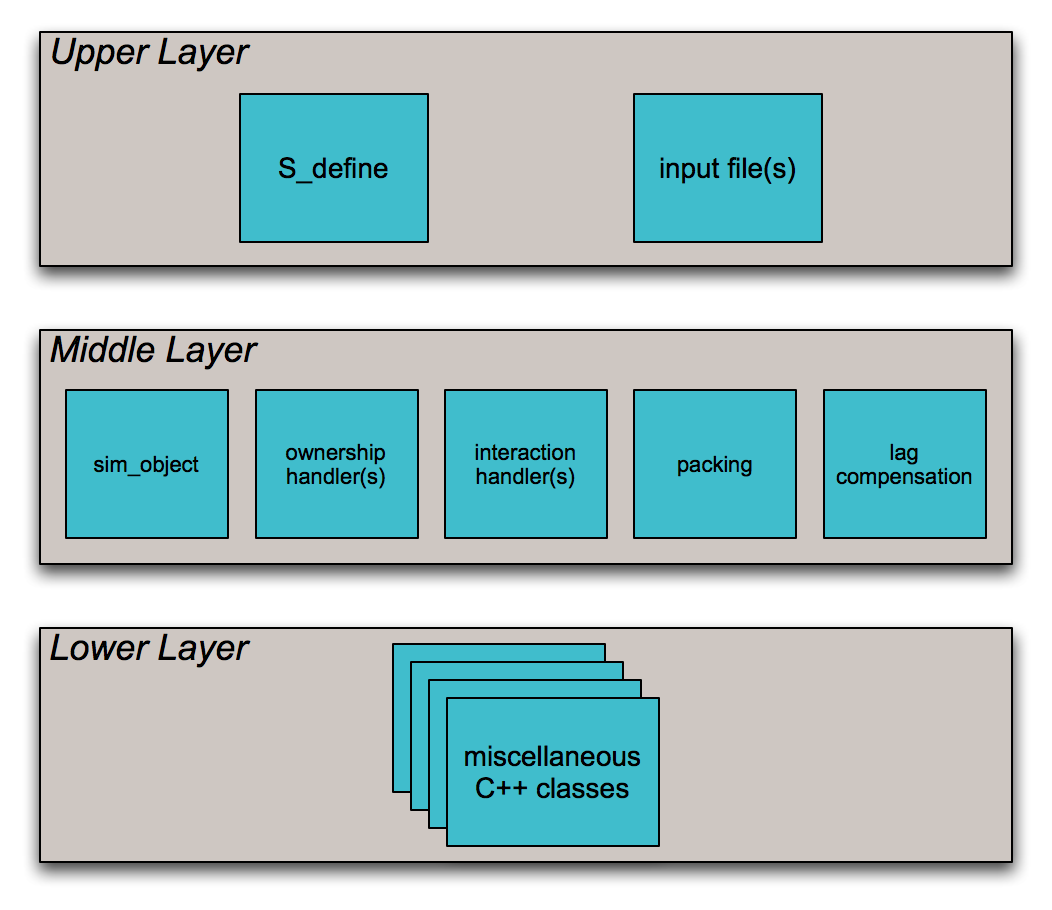
\includegraphics[width=4.5in]{TrickHLA-layers.png}
  \end{center}
\caption{\TrickHLA\ Layers}
\label{fig:TrickHLA-layers}
\end{figure}
%

\subsection{The Upper Layer}

The upper layer of the \TrickHLA\ model consists of simulation-specific
artifacts\footnote{
In a sense, these are not elements of the model, since they are not artifacts delivered 
as part of the model, but since they are important in understanding how the model works, 
we have chosen to explicitly include them in this discussion.}
which must be modified in order to use the model.
These are discussed in the following sections.

\subsubsection{The {\ttfamily S\_define} File}

To integrate \TrickHLA\ into a Trick simulation, the simulation's {\ttfamily S\_define} file
must be modified to include HLA-specific data structures and jobs.
To a large extent, this can be accomplished by inserting the default
\TrickHLA\ {\ttfamily sim\_object} (see below) into the {\ttfamily S\_define} file.
However,
in order to use HLA interactions or ownership management, 
additional {\em handler} data structures (see below) must be inserted into the 
{\ttfamily S\_define} in addition to the {\ttfamily sim\_object}.

\subsubsection{The Input Files}

As discussed on page~\pageref{sec:data-driven-mechanisms},
Trick is a data-driven system. 
Accordingly, most parameters related to the \TrickHLA\ model are initialized 
in the Trick input file fashion.
For example, the name of the federation which the simulation is joining as well as
the hostname and port of the HLA runtime system are specified in input files.
In addition, if the simulation publishes/reflects any simulation data to other federates
or subscribes to data from other federates,
the names of the data are specified in the input files.

\subsection{The Middle Layer}

The model's middle layer consists of the default {\ttfamily sim\_object} and
several other classes that allow developers to customize their handling of 
interactions, ownership transfer, packing and unpacking of transmitted data, 
actions to run upon the deletion of a federate, saving the federation, sending
data conditionally and lag compensation.

\subsubsection{The Default \TrickHLA\ {\ttfamily sim\_object}}

In order to simplify the process of integrating \TrickHLA\ into existing (non-HLA)
simulations,
the model includes a pre-built {\ttfamily sim\_object} which may be inserted into
the {\ttfamily S\_define} verbatim, 
i.e., the HLA-specific data structures and jobs can be mostly contained to this
single object.
The object itself mainly consists of three interrelated data structures and jobs 
related to them:
%
\begin{description}
  \item[TrickHLA::Manager:]{
    This is a C++ class which is mainly responsible for handling the flow of data traffic
    between the core simulation and HLA.
    In particular, it has data structures and methods (which are invoked as jobs)
    responsible for sending and receiving HLA data to/from remote federates.
  }
  \item[TrickHLA::Federate:]{
    This is a C++ class which has methods for coordinating HLA with the Trick
    simulation time and freeze/unfreeze.
    In particular, these methods are responsible for handling HLA time management
    and making sure it is properly synchronized with the simulation time.
  }
  \item[TrickHLA::FedAmb:]{
    This is a C++ class which extends the abstract HLA class,
    {\ttfamily FederateAmbassador}.
    The federate ambassador implements many methods required by the HLA API.
    In particular, the HLA runtime infrastructure asynchronously invokes these methods
    in order to notify the federate that some event occured
    (for example when an object attribute value has been updated by a remote federate).
  }
  \item[TrickHLA::ExecutionControl:]{
    This is a C++ class which extends the abstract \TrickHLA\ class,
    {\ttfamily ExecutionControlBase}.
    This class is used to control the execution of the federate in a defined
    HLA federation execution. This class will implement the execution
    control strategy common to all members of a federation execution.
    \TrickHLA\ provides a muber of available execution control implementations.
    For instance, the SISO standard Space Refernce Federation Object Model
    (SpaceFOM) execution control stategy is provided in the
    {\ttfamily SpaceFOM::ExecutionControl} class.
    
  }
  \item[TrickHLA::ExecutionConfiguration:]{
    This is a C++ class which extends the abstract \TrickHLA\ class,
    {\ttfamily ExecutionConfigurationBase}.
    This class is used to provide configuration data across a coordinated
    federation execution. An execution configuration class is usually paired
    with an execution control class. For instance, the
    {\ttfamily SpaceFOM::ExecutionConfiguration} class is used with the
    {\ttfamily SpaceFOM::ExecutionControl} class.
  }
\end{description}

\subsubsection{Interaction Handlers}

Interactions are not part of the infrastructure in the default {\ttfamily sim\_object}.
In order to send or receive interactions, you must explicitly
insert an interaction handler data structure into the {\ttfamily S\_define} file.
The handler class has a method which may be invoked from the {\ttfamily S\_define} file as a
scheduled job.
The handler is specified in the input file for each interaction the simulation expects
to receive.

\subsubsection{Ownership Handlers}

Ownership transfer is also managed by a handler class.
In order to change ownership of an attribute,
you must explicitly insert an ownership handler data structure into the 
{\ttfamily S\_define} file.
The handler class has methods which ``schedule'' ownership transfers at some future
time. 
By default, no such transfers exist, but by defining one of these ownership handlers
you may arrange for ownership changes using either a {\em push} or {\em pull} model. 
When a push or pull occurs, a job in the default {\ttfamily sim\_object} handles
the low-level details of coordinating the HLA ownership transfer transaction.

\subsubsection{Data Packing and Unpacking}

The \TrickHLA\ model includes an abstract class which may be subclassed by 
simulation developers in order to incorporate simulation-specific packing and unpacking
of data as they arrive from and are sent to remote federates.

\subsubsection{Object Deleted}

The \TrickHLA\ model includes an abstract class which may be subclassed by 
simulation developers in order to incorporate simulation specific action(s), 
which would take place upon the deletion of an object.

\subsubsection{Sending Data Conditionally}

The \TrickHLA\ model includes an abstract class which may be subclassed by 
simulation developers in order to incorporate decision(s) when to send an individual
simulation attribute across the wire. If not overidden, the attribute is sent over the
wire on each data cycle.

\subsubsection{Lag Compensation}

The underlying HLA time management mechanisms involve a protocol which involves 
extrapolation of the system's state forward into the future. 
It is these forward predictions of the system state that are sent to remote federates.
This mechanism is what permits the distributed federates to operate concurrently 
but at the same time maintain a consistent notion of the current simulation time.
However, protocol introduces simulation-time lags in the data each time attribute
ownership is transfered from one federate to another.
In order to compensate for this lag, sending or receiving federates may subclass
an abstract lag compensation class included in the \TrickHLA\ model.
This class includes methods that act as hooks allowing the federates to 
extrapolate the state in time in order to compensate for the protocol-introduced
time lag.

\subsection{The Lower Layer}

This layer consists of a number of C++ classes that implement HLA constructs such as
objects, attributes, interactions, parameters, and synchronization points.
In addition there are some low level classes that serve primarily to hold utility methods,
e.g., string and byte-swapping methods.

